\documentclass[border=5pt]{standalone}
\usepackage{tikz}
\usepackage{xcolor}
\usetikzlibrary{calc,shadows.blur}

% J9 - Pink flanged disk with holes
\begin{document}
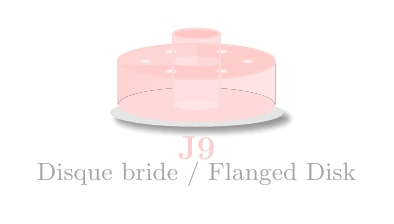
\begin{tikzpicture}

% Shadow
\fill[gray!20,blur shadow={shadow blur steps=5}] (0,-0.5) ellipse (1.1 and 0.18);

% Bottom ellipse
\fill[pink!60] (0,-0.4) ellipse (1.0 and 0.22);
% Center hub bottom
\fill[pink!40] (0,-0.4) ellipse (0.3 and 0.066);

% Flange side wall
\fill[left color=pink!70, right color=pink!40]
  (-1.0,-0.4) -- (-1.0,0.15) arc[start angle=180,end angle=0,
  x radius=1.0,y radius=0.22] -- (1.0,-0.4)
  arc[start angle=0,end angle=180,x radius=1.0,y radius=0.22];

% Hub cylinder wall
\fill[pink!50]
  (-0.3,-0.4) -- (-0.3,0.5)
  arc[start angle=180,end angle=0,x radius=0.3,y radius=0.066]
  -- (0.3,-0.4)
  arc[start angle=0,end angle=180,x radius=0.3,y radius=0.066];

% Top flange face
\fill[pink!80] (0,0.15) ellipse (1.0 and 0.22);
\fill[pink!60] (0,0.15) ellipse (0.3 and 0.066);

% Top hub face
\fill[pink!90] (0,0.5) ellipse (0.3 and 0.066);

% Bolt holes on flange top (6 holes)
\foreach \angle in {0,60,120,180,240,300}{
  \fill[pink!20] ({0.65*cos(\angle)},{0.15+0.65*0.22*sin(\angle)}) ellipse (0.07 and 0.02);
  \draw[pink!50,thin] ({0.65*cos(\angle)},{0.15+0.65*0.22*sin(\angle)}) ellipse (0.07 and 0.02);
}

% Highlight
\begin{scope}
  \clip (0,0.15) ellipse (1.0 and 0.22);
  \fill[white,opacity=0.2] (-1.1,0.1) rectangle (0.0,0.4);
\end{scope}

% Outlines
\draw[pink!70, line width=0.8pt] (0,0.15) ellipse (1.0 and 0.22);
\draw[pink!60, line width=0.7pt] (0,0.5) ellipse (0.3 and 0.066);
\draw[pink!60, line width=0.7pt] (-0.3,-0.4)--(-0.3,0.5);
\draw[pink!60, line width=0.7pt] (0.3,-0.4)--(0.3,0.5);

% Label
\node[font=\bfseries\large, text=pink!80] at (0,-0.95) {J9};
\node[font=\small, text=gray!70] at (0,-1.28) {Disque bride / Flanged Disk};

\end{tikzpicture}
\end{document}
